%%%%%%%%%%%%%%%%%%%%%%%%%%%%%%%%%%%%%%%%%%%%%%%%%%%%%%%%%
%                                                       %
%  情報処理学会全国大会投稿論文用テンプレートファイル   %
%                   for ips.sty ver2.1                  %
%                                                       %
%%%%%%%%%%%%%%%%%%%%%%%%%%%%%%%%%%%%%%%%%%%%%%%%%%%%%%%%%

%%% ver2.1 +
%%% edited by Jutori
%%% modified by Kenta

\documentclass[a4paper,9pt, twocolumn]{jarticle}
% pngなどをそのまま使うためのusepackage
\usepackage[dvipdfmx]{graphicx}
\usepackage{bmpsize}
% [H]などで位置調整するためのusepackage
\usepackage{float}
% 表関連
\usepackage{amssymb, amsmath}
\usepackage{booktabs}
% コードブロック関連 jlistingにより日本語コメントアウトでも崩れないようにできる
\usepackage{listings,jlisting,here}
% キャプション用パッケージ
\usepackage{caption}
% コードの書式
\lstset{
    basicstyle={\scriptsize\ttfamily},
    identifierstyle={\scriptsize},
    commentstyle={\scriptsize\itshape},
    keywordstyle={\scriptsize\bfseries},
    ndkeywordstyle={\scriptsize},
    stringstyle={\scriptsize\ttfamily},
    frame={tb},
    breaklines=true,
    columns=[l]{fullflexible},
    numbers=left,
    xrightmargin=0zw,
    xleftmargin=3zw,
    numberstyle={\tiny},
    stepnumber=1,
    numbersep=1zw,
    lineskip=-0.5ex,
    captionpos=b
}
% ソースコードと図番号を共通の連番にする
\makeatletter
\AtBeginDocument{%
	\let\c@figure\c@lstlisting
	\let\thefigure\thelstlisting
	\let\ftype@lstlisting\ftype@figure
}
\makeatother
\makeatletter
\AtBeginDocument{
	\renewcommand*{\thelstlisting}{\arabic{lstlisting}}
	% \@addtoreset{lstlisting}{chapter}
}
\makeatother
\renewcommand{\lstlistingname}{図} % ソースコードでなく図とする

\newcommand{\ri}[1]{図 \ref{#1}}
\newcommand{\ti}[1]{表 \ref{#1}}

%\documentclass[a4paper,9pt,twocolumn]{ipsjpapers}
\usepackage{ips}
\usepackage{mediabb}

\renewcommand{\baselinestretch}{0.87}   % 行間

\pagestyle{empty}
%%%%%%    TEXT START    %%%%%%
\begin{document}

%%%%%%%%%%%%%%%%%%%%%%%%%%% ヘッダ %%%%%%%%%%%%%%%%%%%%%%%%%%
\twocolumn[%
	\begin{center}

		%--------------------------------------------------------------
		% 講演タイトル(2行にわたるときは\2jtitle{}{}{})
		%--------------------------------------------------------------

		\vspace{-3mm}
		\jtitle{「改訂版ブルーム・タキソノミー」を利用した}
		\jtitle{ソフトウェアドキュメンテーションの改善手法の提案}

		%--------------------------------------------------------------
		% 日本語著者名
		%--------------------------------------------------------------
		% name{1}{***} : 所属1の氏名
		% name{2}{***} : 所属2の氏名 のようにする.所属の引数は4まで
		% 名前は絶対間違えないように

		\begin{authors}
			\name{1}{山川 陽亮}
			\name{2}{金城 篤史}
		\end{authors}
		%--------------------------------------------------------------
		% 所属
		%--------------------------------------------------------------
		% aff{1}{***} : 所属1
		% aff{2}{***} : 所属2 のようにする.所属の引数は4まで.

		\begin{affiliation}
			\aff{1}{ピクシブ株式会社}
			\aff{2}{沖縄工業高等専門学校}
		\end{affiliation}

		%--------------------------------------------------------------
	\end{center}
]%

%%%%%%%%%%%%%%%%%%%%%%%%    脚注   %%%%%%%%%%%%%%%%%%%%%%%%%%

%--------------------------------------------------------------
% 英文タイトル
%--------------------------------------------------------------

\etitle{Applying the Revised Bloom's Taxonomy to Improve Software Documentation}


%--------------------------------------------------------------
% 英語語著者名
%--------------------------------------------------------------
% ename{1}{***} : 所属1の氏名
% ename{2}{***} : 所属2の氏名 のようにする.

\ename{1}{Yosuke Yamakawa}
\ename{2}{Atsushi KINJO}
%ename{2}を使う場合,所属1の人と2の人で改行されてしまうので,\enameをコメントアウトして以下のように直接書くのをおすすめ (空白は適宜調節のこと)
%ただし所属が3の場合は†††でなく‡となるので,\ddagと付けること
%\footnotetext{%
%    \hspace{-3mm}\raise1ex\hbox{{\scriptsize \dag}}First Last,%
%    \hspace{1.5mm}\raise1ex\hbox{{\scriptsize \dag}}First Last,%
%    \hspace{1.5mm}\raise1ex\hbox{{\scriptsize \dag\dag}}First Last,%
%    \hspace{1.5mm}\raise1ex\hbox{{\scriptsize \ddag}}First Last,%
%}
%\footnotetext{%
%    \hspace{-1mm}\raise1ex\hbox{{\scriptsize \dag\dag}}First Last and%
%    \hspace{1mm}\raise1ex\hbox{{\scriptsize \dag\dag}}First Last%
%}


%--------------------------------------------------------------
% 英語所属
%--------------------------------------------------------------
% eaff{1}{***} : 所属1
% eaff{2}{***} : 所属2 のようにする.所属の引数は4まで.
% ※日本語の所属と対応させること.
\eaff{1}{pixiv Inc.}
\eaff{2}{Okinawa National College of Technology}


%--------------------------------------------------------------
% 英語住所
%--------------------------------------------------------------



% 上マージン30mm 下25mm 横20mm 段組の間隔 7mm
% 印刷した後,自分で確認すること

%%%%%%%%%%%%%%%%%%%%%%%% ここから本文 %%%%%%%%%%%%%%%%%%%%%%%%%%
% 脚注番号は数字で振る
\renewcommand{\thefootnote}{*\arabic{footnote}}
% !TEX root = ../zenkoku.tex
\section{はじめに}
ソフトウェア開発において,チーム内で熟練した開発者(以降,熟練者)はドキュメントを作成することがある.\cite{bib:ozawa}

% FIXME: なんか構造がおかしい,どのドキュメントに焦点を当てるかはもっと簡潔にかつ後に触れたほうが良さそう
% そもそも説明したいことに対して文量が多すぎるように思える
ソフトウェア開発におけるドキュメントには,会社等の組織の中で開発されるシステムに対するドキュメント,OSS開発プロジェクトで開発されるシステムのドキュメント,ある組織が別の組織・個人に対して公開する開発者向けSDKに対するドキュメントなど複数の状況・用途が考えられるが,今回は山川が所属する株式会社の事業部の開発組織で開発・運用している広告配信システムの各サブシステム\footnote{全社共通で使われるようなシステムやツールではない}を対象に,熟練者が社内の他の開発者向に対し知識の共有を目的として作成するドキュメントに焦点を当てる.

情報工学においてはドキュメントを作成しなければいけない状況が存在するが,ドキュメントを執筆することで開発者が実装等に使えた時間は減ることになってしまう.
またドキュメントは充足したという状況を測ることが難しい,ドキュメント化対象のシステムが多すぎる,などの問題も存在する.
知識の共有を目的としてドキュメントが作成されるのであれば,熟練者への属人性が高いサブシステムに対してドキュメントが無いものを洗い出すことでドキュメント化対象を絞ること,優先度を付けることが可能なのではないかと考えた.

% FIXME: 前の分との繋がりが不自然,もう少し丁寧な導入無いかな
% FIXME: 「知識の呪縛」という概念はここ以降で使うつもりがないので出来れば用語を出さずに概念だけ説明して,残りは引用元を参照してね,という形にしたい
教育学における「知識の呪縛」(すでに理解した情報を知らないものととして想定することは難しいこと)\cite{bib:kaneda}は情報工学においても起きていることなのではないかと考える.例えば,熟練者が執筆したドキュメントは他の開発者にとって十分な情報を満たしたものとならない(知識の呪縛による認知バイアスがかかるため)などが挙げられる.

% FIXME: この段落が前の段落から飛躍しすぎているように感じる
ドキュメントが良いものであれば,ドキュメントが対象とする人の理解度が上がると考えられる.そこで本稿では,ドキュメント作成前にドキュメント対象者の理解度を計測し,これを元にドキュメントを作成する.

ただ理解度は個人の認知に基づく指標であるため,本稿では教育心理学にて知られている改訂版ブルーム・タキソノミー\cite{bib:nakao}という枠組を使い,理解度の数値化を行う.

\section{理解度を計測する指標}
理解度を個人の認知だけではなく,指標を元に多角的に評価するための枠組みは複数あるが,そのうちの1つであり教育学にて用いられることのある「改訂版ブルーム・タキソノミー」\cite{bib:anderson}に注目することにする.

ブルーム・タキソノミーでは,学習者の行動を認知的領域,情意的領域,精神運動的領域の3つに分類する.
このうち認知的領域は,記憶,理解,応用,分析,評価,創造,の6段階に分けられる.

本稿では,この6段階の認知段階を情報工学に適用し,認知レベルを理解度を示す指標として用いて活用することを目指す.実装としてはこれに基づいたアンケート作成する.
作成したアンケートをドキュメント利用者に回答してもらい認識を測定する.
測定結果をドキュメント作成者へフィードバックし,熟練者と他の開発者の間に生じる認識齟齬を改善することを目指す.

本稿ではシステムに対する理解度(自己認識)をアンケートによって回答してもらい,その結果を元にドキュメンテーションに役立てる


% !TEX root = ../zenkoku.tex
\section{アンケートの内容}
アンケートの内容は以下の通りである\newline

このサービスについてこれまでの質問を踏まえあなたの理解を教えて下さい\footnote{これより前にアンケートの回答を円滑にするためにシステムに対する設問を行っているが,本稿ではブルーム・タキソノミーを元に作成した設問のみ扱う}\footnote{アンケートの選択肢には「認識・記憶できる」の前の段階として「認識・記憶できない」を追加した}\newline

(注釈)
\begin{itemize}
    \item 1~6のうち6に近いほど理想の状態だと考えてください
    \item 「認識・記憶できる」のうち例に挙げられている項目のすべてを満たさなくても「認識・記憶できる」に該当する場合はありえます。下記文章はあくまで参考程度に考えてください
\end{itemize}
(理解度を選択するための具体例)\footnote{アンケートでは以下の例に追加でもう2個ほど例示がある}

\renewcommand{\arraystretch}{1.5} % 表の隙間がデフォルトだと小さすぎるので標準の1.5倍にする
\scriptsize
% カウンタを作成
\newcounter{rownumber}

\begin{tabular}{|p{2.5cm}|p{4.2cm}|}
    \hline
    \textbf{レベル} & \textbf{説明と例} \\
    \hline
    \stepcounter{rownumber}\arabic{rownumber}. 認識・記憶できる & ツール上の情報を認識し利用する \newline 例:このツールで特定のCPU使用率のグラフを見つけられる など \\
    \hline
    \stepcounter{rownumber}\arabic{rownumber}. 理解できる & 情報を解釈し、説明や比較ができる \newline 例:各モジュールが何を担当しているか説明できる など \\
    \hline
    \stepcounter{rownumber}\arabic{rownumber}. 応用できる & 学んだ知識を具体的な状況で使える \newline 例:新しいパラメータをAPIに追加し、動作確認ができる など \\
    \hline
    \stepcounter{rownumber}\arabic{rownumber}. 分析できる & 情報を分解し、要素間の関係を理解できる \newline 例:エラー発生原因をログやコードベースから特定できる など \\
    \hline
    \stepcounter{rownumber}\arabic{rownumber}. 評価できる & 批判的に情報を評価し、結論を導き出せる \newline 例:新しい要件を検討し、それが現在のアーキテクチャに適合するかを判断できる など \\
    \hline
    \stepcounter{rownumber}\arabic{rownumber}. 創造できる & 新しいアイデアや設計を作り出せる \newline 例:大規模な変更を伴う新しい機能を提案し、それを設計・実装できる など \\
    \hline
\end{tabular}

\normalsize % 他の部分の文字サイズを元に戻す

% TODO: 少し文章直す

理解度を選択するための具体例がアンケート上に書いてあり,それをもとにアンケート回答者が1~6の理解度を自分で選択している.
他人に評価されるわけではない.


% !TEX root = ../zenkoku.tex
\section{アンケートの対象とするシステム}
今回のアンケートでは筆者の所属する開発組織で開発・運用をこなっている21個のシステム,6個のツール,2個のインフラに関する設問を設定した.


% !TEX root = ../zenkoku.tex
\section{アンケート対象者}
アンケートの対象者は筆者の所属する開発組織で開発・運用を行っている9人の開発者となる.
これらのアンケート回答者はブルーム・タキソノミーについての事前知識が与えられないままアンケートを回答している.


% !TEX root = ../zenkoku.tex
\section{結果}
アンケートは部の開発者全員である9人全員から回答を得た.

集計方法としては熟練した開発者を1人想定し,この開発者への依存度が高いようなシステムを洗い出すことにした.
`熟練者の理解度 - 熟練者を除いた平均` によって求めた数値を属人性の高さとする.

結果を表hogeに示す
% ここヒストグラム書いても良いかも.線の値が大きくなるほど属人性が高いもの

表1.属人性の高さ
memo: 右側の個別の開発者のやつ消す
memo: 認識で0を選択した人は省く,開発に関わっていない人も含まれてしまう



% !TEX root = ../zenkoku.tex
\section{結果}
熟練者がチームに1人いる状況を想定し,結果から熟練者への依存度が高いようなシステムを洗い出すことにした.
熟練者としては,アンケートの対象とする各サブシステムに直近1年間最も多くデプロイした開発者,新機能の実装やコードベースの管理に多く取り組んだ開発者,について総合的に判断し,当てはまる上位1人を今回の考察の対象とした.
またこれらの指標はOSS (Open Source Software) 開発プロセスに関する研究\cite{bib:mockus}におけるコア開発者の指標を参考にした.

アンケートの結果を\ri{img:rikai}に示す.

\begin{figure}[h]
	\centering
	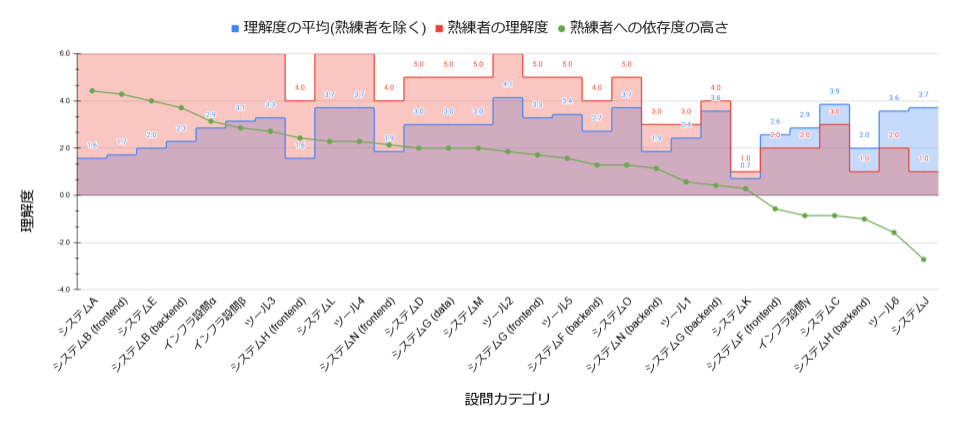
\includegraphics[keepaspectratio,width=0.9\linewidth]{img/rikai.png}
	\caption{理解度の平均と熟練者への依存度の高さ}
	\label{img:rikai}
\end{figure}

理解度は値が高いほど理解が深いものとし,`熟練者の理解度 - 熟練者を除いた回答者の理解度平均` によって求めた数値を熟練者への依存度の高さとする.
縦軸がブルーム・タキソノミーでの理解度,横軸が設問カテゴリ(各サブシステム)となっている.
また重ね合わせられている棒グラフは熟練者への依存度の高さを表している.
各設問カテゴリの順番は左から熟練者への依存度の高い順に並べている.

また,この結果をアンケートを回答した開発組織のエンジニアに対し討論する機会を設けたところ,「この結果が示す理解度の平均・熟練者への依存度の高さ共に認識と相違ない」という意見が得られた.


\renewcommand{\baselinestretch}{0.83}\selectfont
\vspace{-0.5mm}

%
% ------ 参考文献 ------
%
\begin{thebibliography}{9}
	\itemsep -1.7pt

	\bibitem{bib:ozawa}
	{\small '小沢 暢, 松野 裕':
	\newblock ソフトウェア開発プロジェクトにおける引き継ぎプロセス及びドキュメント作成手順の提案と評価,
	\newblock 実践的IT教育シンポジウム rePiT 論文集,
	\newblock Vol.2023,
	\newblock No.0,
	\newblock pp.93-100,
	\newblock 2023.}

	\bibitem{bib:kaneda}
	{\small '金田 茂裕':
		\newblock 教授者の課題知識と学習過程知識が教授学習法の望ましさ判断に及ぼす影響,
		\newblock 教育心理学研究,
		\newblock Vol.70,
		\newblock No.4,
		\newblock pp.333-346,
		\newblock 2022.}

	\bibitem{bib:anderson}
	{\small 'Anderson, Lorin W., Krathwohl, David R., Bloom, Benjamin Samuel':
		\newblock A taxonomy for learning, teaching, and assessing: a revision of Bloom's taxonomy of educational objectives,
		\newblock 2001.}

	\bibitem{bib:nakao}
	{\small 中尾 桂子:
		\newblock「発問」に基づく授業デザイン振り返りの試み : 改訂版タキソノミーを援用した教師のためのCan-Doリストの開発にむけて,
		\newblock 大妻女子大学紀要. 文系 = Otsuma Women's University annual report. Humanities and social sciences,
		\newblock Vol.52,
		\newblock pp.185–200,
		\newblock 2020.}

	\bibitem{bib:miyahara}
	{\small '宮原 史, 堤 盛人':
		\newblock 戦略的な人材育成の実現に向けた道路橋を維持管理する技術力の解明の試み ―ブルーム・タキソノミーの応用―,
		\newblock 土木学会論文集F4(建設マネジメント),
		\newblock Vol.76,
		\newblock No.1,
		\newblock pp.14-28,
		\newblock 2020.}

\end{thebibliography}

\end{document}
